% !Mode:: "TeX:UTF-8"
\chapter{可见光多波段OFDM系统的信道估计}
\section{引言}
所谓信道估计,就是在接收端估计出信道状态信息(Channel State Information,CSI),为下一步地解调做准备,也是自适应传输技术的基础。无线通信一个重要的特征就是发射端到接收端之间的路径比较复杂,不像有线通信那样是固定且可预知的,所以信道估计技术在无线通信领域格外重要,特别是在OFDM 等需要相干检测的系统中。本章将着重介绍信道估计技术,首先介绍传统射频通信中OFDM 系统的信道估计方法,然后具体到可见光通信系统中的信道估计问题,再将结合实际系统设计,讨论信道的非线性问题,最后将研究多色可见光通信系统中各波段之间串扰的估计。
\section{OFDM信道估计常用方法}
信道估计总体可以分为两大类,盲信道估计和基于导频的信道估计。盲信道不需要额外的导频或者训练序列,因此频率利用率高;但是它的缺点是计算量大、算法复杂,而且精度低、收敛速度缓慢,难以用于移动通信环境
\cite{石钧2012ofdm}。基于导频的信道估计原理是在发射端插入专门用于信道估计的导频或者训练序列,并且这些序列对于接收端也是已知的,接收端根据接收到的经过了信道后的导频序列与原导频序列之间的关系,估计出信道冲击响应(Channel Impulse Response,CIR)。这类信道估计方法因为要插入导频序列会稍微降低整个系统的传输速率,但是其估计实现复杂度低、估计精度高,在实际工具中大都采用这种方法。本节也主要讨论基于导频的信道估计算法。
\begin{figure}[htbp]
    \centering
    \subfloat[块状导频放置方式]{
        \label{fig:BlockTypePilot}
        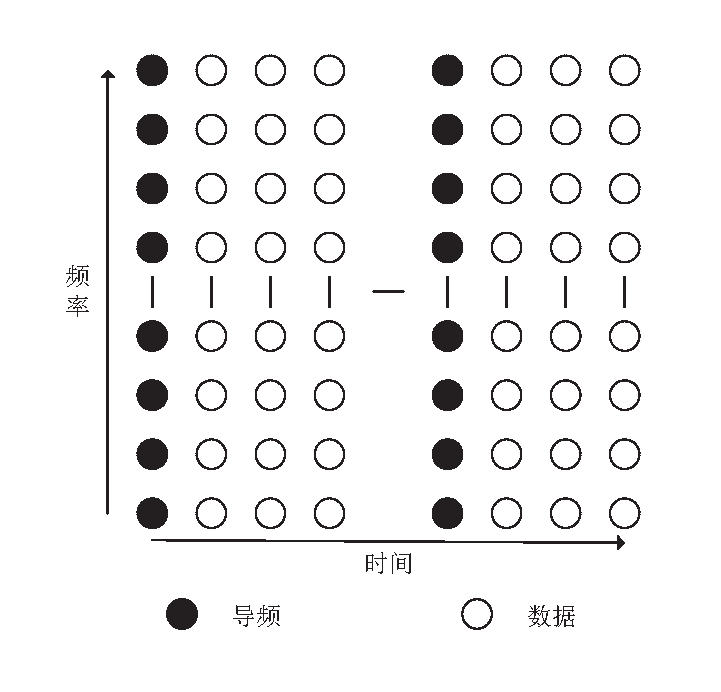
\includegraphics[width = 0.5\textwidth]{figures/Chapter-3/BlockTypePilot.eps}
    }
    \subfloat[梳状导频放置方式]{
        \label{fig:CombTypePilot}
        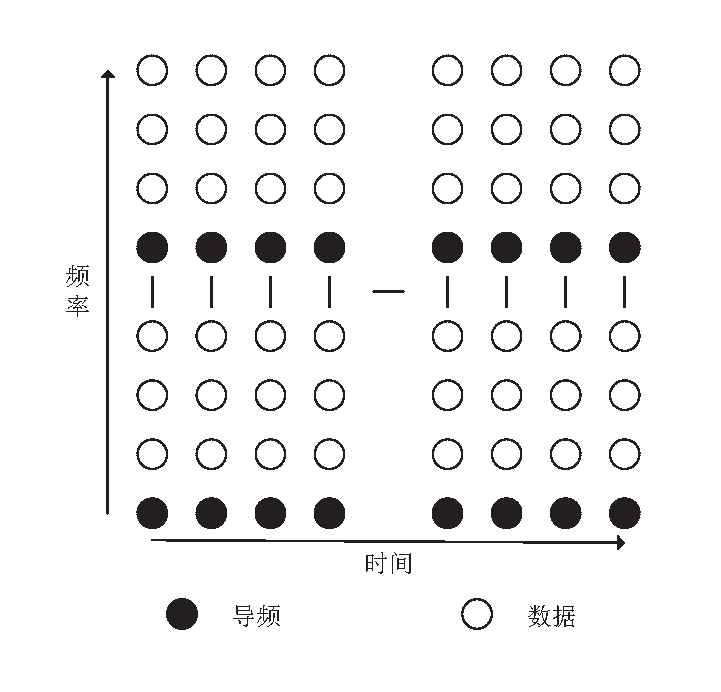
\includegraphics[width = 0.5\textwidth]{figures/Chapter-3/CombTypePilot.eps}
    }
    \caption{导频放置方式}
    \label{fig:PilotAllocation}
\end{figure}






\section{可见光信道估计}
\section{可见光信道非线性分析}
\section{可见光各波段之间串扰估计}
\section{本章小结}
